\documentclass[tikz]{standalone}

\usetikzlibrary{decorations.pathmorphing,patterns,calc}

\begin{document}
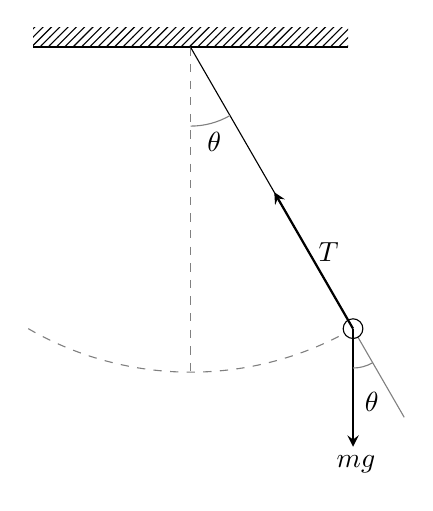
\begin{tikzpicture}
\def\centerarc[#1](#2)(#3:#4:#5)% Syntax: [draw options] (center) (initial angle:final angle:radius)
	{ \draw[#1] ($(#2)+({#5*cos(#3)},{#5*sin(#3)})$) arc (#3:#4:#5); }
	\coordinate (extreme) at (-60:4);
	\coordinate (ball) at (-60:4.125);
	
	%Roof
	\fill [pattern = north east lines] (-2,0) rectangle (2,0.25);
	\draw[thick] (-2,0) -- (2,0);
	
	%Dashed lines
	\draw[gray, dashed] (0,0) -- (0,-4.125);
	%\draw[gray, dashed] (-2,-3.4) arc(-120:-60:4);
	\centerarc[gray,dashed](0,0)(-120:-60:4.125)

	%Rope
	\draw (0,0) -- (extreme);
	
	%Axis
	%\draw[gray] (ball) -- ++(30:1) -- ++(180 + 30:2);
	\draw[gray] (ball) -- ++(-60:1.3);
	
	%Ball
	\draw[fill=white] (ball) circle (0.125);
	
	%Forces
	\draw[-stealth, thick] (ball) -- ++(-90:1.5);
	%\draw[-stealth, thick] (ball) -- ++(-60:1.5*0.867);
	%\draw[-stealth, thick] (ball) -- ++(-90-60:1.5*0.5);
	
	\draw[-stealth, thick] (ball) -- ++(120:2);
	\node[right] at (-60:3) {$T$};
	
	%Angles
	\centerarc[gray](ball)(-90:-60:0.5)
	\node at (0.3, -1.2) {$\theta$};
	\centerarc[gray](0,0)(-90:-60:1)
	\node at (2.3, -4.5) {$ \theta $};
	
	%Text
	%\node[rotate=-60] at (2.6,-4) {$mg \cos{\theta}$};
	\node at (2.1, -5.3) {$mg$};
	%\node[rotate=30] at (1.2, -3.7) {$mg \sin{\theta}$};
\end{tikzpicture}

\end{document}